%New colors defined below
\definecolor{codegreen}{rgb}{0,0.6,0}
\definecolor{codegray}{rgb}{0.5,0.5,0.5}
\definecolor{codepurple}{rgb}{0.58,0,0.82}
\definecolor{backcolour}{rgb}{0.95,0.95,0.92}

%Code listing style named "mystyle"
\lstdefinestyle{mystyle}{
  backgroundcolor=\color{backcolour},   commentstyle=\color{codegreen},
  keywordstyle=\color{magenta},
  numberstyle=\tiny\color{codegray},
  stringstyle=\color{codepurple},
  basicstyle=\footnotesize,
  breakatwhitespace=false,
  breaklines=true,
  captionpos=b,
  keepspaces=true,
  numbers=left,
  numbersep=5pt,
  showspaces=false,
  showstringspaces=false,
  showtabs=false,
  tabsize=2
}

%"mystyle" code listing set
\lstset{style=mystyle}

\section{PostgreSQL}
La instalación se llevará por medio de la consola del sistema operativo (Ubuntu), por lo que primero debe acceder a la misma por medio de la combinación de teclas Ctrl + Alt + T.

\begin{figure}[H]
  \begin{center}
    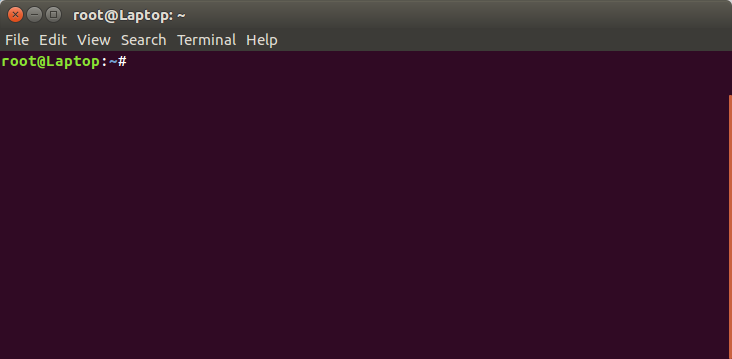
\includegraphics[scale=0.35]{images/INST/1.png}
    \caption{Terminal del sistema.}
  \end{center}
\end{figure}

\subsection{Purga del sistema}

Al inicio es necesario remover cualquier posible versión que exista en el sistema que pueda entrar en conflicto con la que se intenta instalar, para ello debe ejecutar los siguientes comandos.
\bigbreak
En primer lugar, detiene los posibles servicios relacionados en ejecución.

\begin{lstlisting}[language=bash]
    /etc/init.d/postgresql stop
    sudo systemctl stop postgresql.service
\end{lstlisting}

\begin{figure}[H]
	\begin{center}
		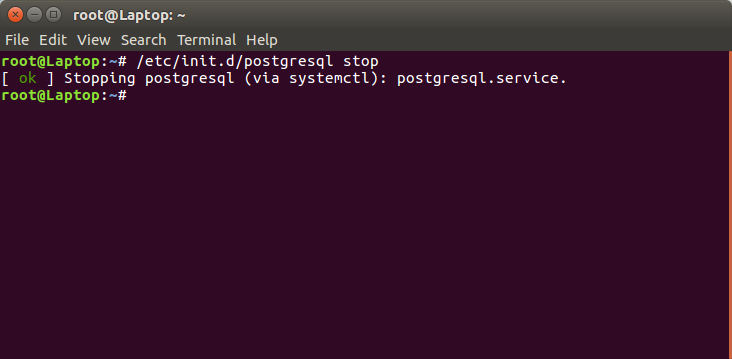
\includegraphics[scale=0.35]{images/INST/2.png}
		\caption{Mensaje de confirmación de la detención del servicio.}
	\end{center}
\end{figure}

\bigbreak
A continuación, elimina los archivos y ficheros relacionados.

\begin{lstlisting}[language=bash]
    sudo apt-get --purge remove postgresql\*
    sudo rm -r /etc/postgresql/
    sudo rm -r /etc/postgresql-common/
    sudo rm -r /var/lib/postgresql/
    sudo userdel -r postgres
    sudo groupdel postgres
    sudo apt-get remove --auto-remove pgadmin4
\end{lstlisting}

\begin{figure}[H]
	\begin{center}
		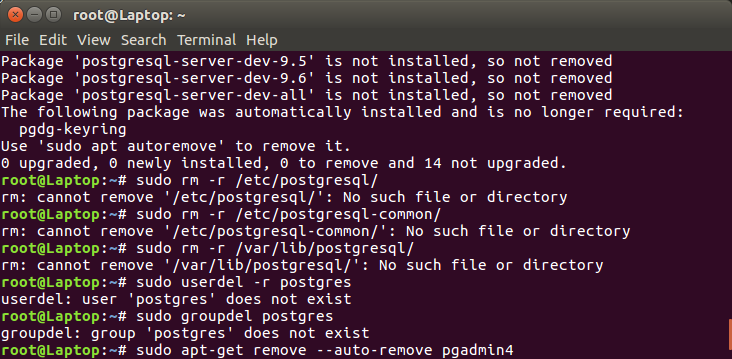
\includegraphics[scale=0.35]{images/INST/3.png}
		\caption{Purga del sistema.}
	\end{center}
\end{figure}

\bigbreak
Procede a descargar e instalar PostgreSQL, así como PGAdmin4 que será el administrador auxiliar.

\subsection{Instalación}
\begin{lstlisting}[language=bash]
    sudo apt-get update
    sudo apt-get install postgresql postgresql-11
    sudo apt-get install pgadmin4
\end{lstlisting}

\begin{figure}[H]
	\begin{center}
		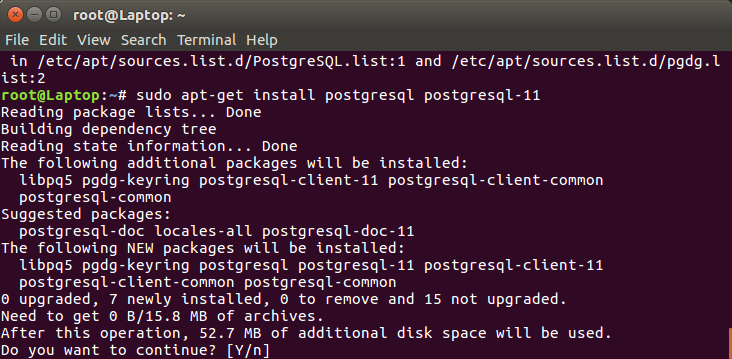
\includegraphics[scale=0.35]{images/INST/4.png}
		\caption{Instalación PostgreSQL.}
	\end{center}
\end{figure}

\bigbreak
\subsection{Verificación}

Lo siguiente es verificar si se instaló correctamente el Adminsitrador de Base de Datos, para ello ejecuta el siguiente comando y debe aparecer la versión instalada previamente.
\begin{lstlisting}[language=bash]
    psql --version
\end{lstlisting}

\begin{figure}[H]
	\begin{center}
		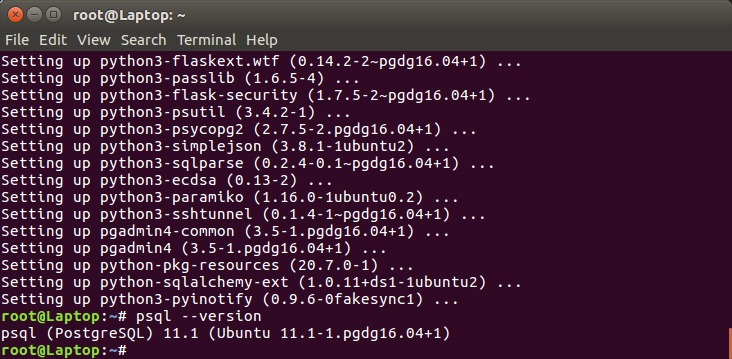
\includegraphics[scale=0.35]{images/INST/5.png}
		\caption{Verificación instalación.}
	\end{center}
\end{figure}

\bigbreak
\subsection{Configuración del Sistema}

Una vez instalado el Administrador de la Base de Datos, procede a configurar el sistema por medio de la creación de un usuario específico que llevará los procesos relacionados a la Base de Datos para posteriormente incializar la misma.

\subsection{Creación del usuario}

Añade un usuario tipificado como 'postgres', la contraseña que le colocará será la que se le proporcione al momento de hacerle entrega del sistema.

\begin{lstlisting}[language=bash]
    sudo passwd postgres
\end{lstlisting}

\begin{figure}[H]
	\begin{center}
		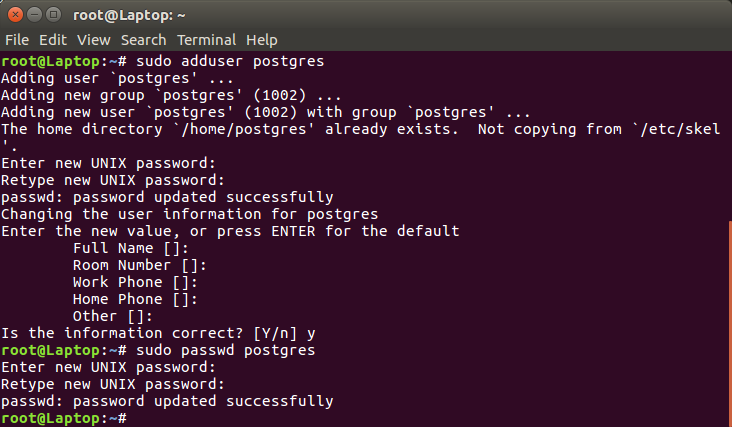
\includegraphics[scale=0.35]{images/INST/6.png}
		\caption{Creación del usuario.}
	\end{center}
\end{figure}

\subsection{Acceso al usuario}

A modo de verificación de lo anterior, así como paso intermedio para los subsecuentes, inicia los servicios del Administrador de la Base de Datos y accede al usuario recién creado.

\begin{lstlisting}[language=bash]
    sudo systemctl start postgresql.service
    sudo -i -u postgres
\end{lstlisting}

\begin{figure}[H]
	\begin{center}
		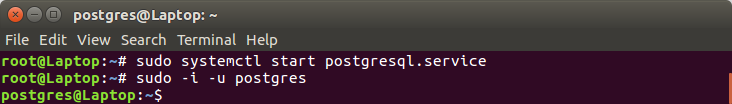
\includegraphics[scale=0.35]{images/INST/7.png}
		\caption{Acceso al usuario.}
	\end{center}
\end{figure}

\subsection{Acceso a PostgreSQL}

Establece los permisos para el perfil Administrador de la Base de Datos.

\begin{lstlisting}[language=bash]
    psql
\end{lstlisting}
\begin{lstlisting}[language=SQL]
    ALTER USER postgres PASSWORD 'root';
    create database apms;
    \c apms
\end{lstlisting}

\begin{figure}[H]
	\begin{center}
		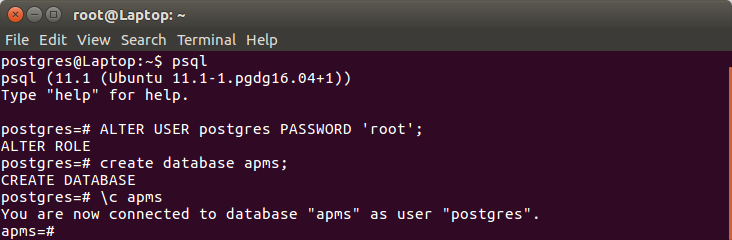
\includegraphics[scale=0.35]{images/INST/8.png}
		\caption{Establecimiento de permisos para la Base de Datos.}
	\end{center}
\end{figure}